\documentclass[11pt]{article}
\title{Meccano pentagons gallery}
\author{https://github.com/heptagons/meccano/penta}
\date{}

%\usepackage{gallery/penta}
%\usepackage{longtable}
\usepackage{../meccano}
\begin{document}

\maketitle
\begin{abstract}
We show constructions of small meccano pentagons.
\end{abstract}

\section{Pentagon size 12}

\begin{figure}[htp]
 \centering
 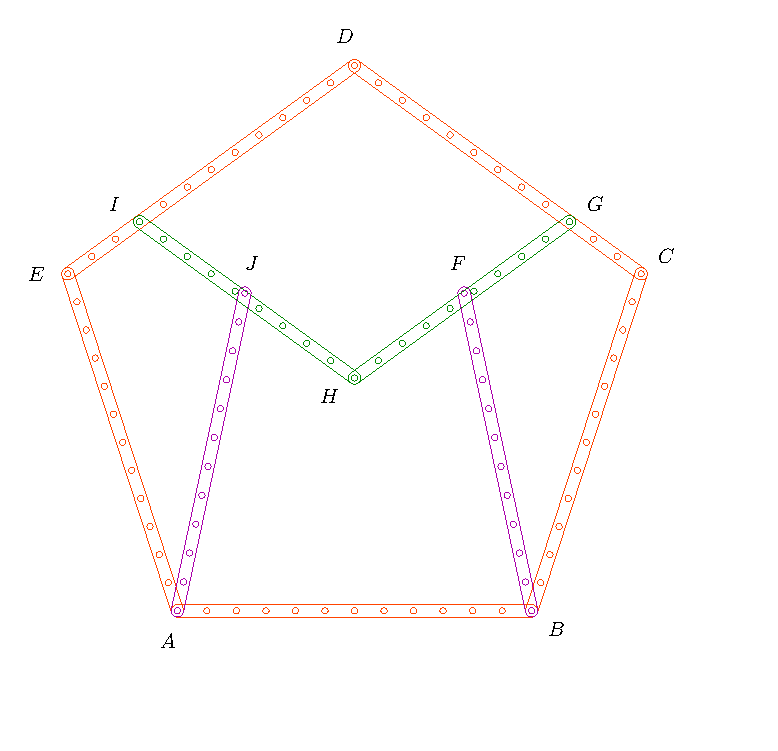
\includegraphics[scale=0.75]{gallery/penta12a}
 \caption{Pentagon size 12.}
 \label{fig:penta12a}
\end{figure}

From figure \ref{fig:penta12a} we have the regular pentagon of side 12 $A,B,C,D,E$.


\end{document}